%Différente classes qui intéragissent ensemble

Totoscope est donc un logiciel de rotoscopie utilisant la librairie Qt. Nous avons donc essayer d'utiliser les fonctionnalités de cette librairie au mieux.

Notre logiciel est composé de plusieurs fenêtres, nous allons  décrire les fonctionnalités et les choix opérés pour chaque fenêtre.

\subsection{Fenêtre d'ouverture}

	\begin{figure}[!h]
		\centering
		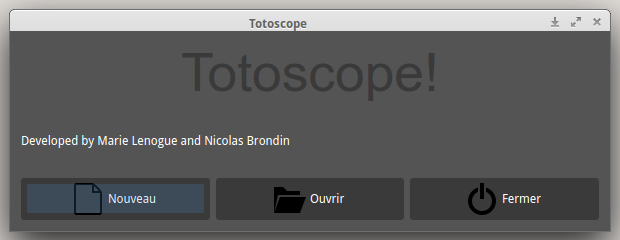
\includegraphics[scale=0.5]{./figures/opening.png}
		\caption{Fenêtre d'ouverture du logiciel}
	\end{figure}

	La fenêtre d'ouverture offre plusieurs possibilités à l'utilisateur : 
	
	\subsubsection*{La création d'un nouveau projet}
			Le choix de cette option, vous ouvre une nouvelle fenêtre permettant d'entrer le nom du projet désiré, la vidéo que l'on souhaite traiter ainsi que le nombre d'images par seconde voulu.
			
			\vspace{0,5cm}
			
	\begin{figure}[h]
		\centering
		
\includegraphics[scale=0.5]{./figures/new.png}
		\caption{Fenêtre de création d'un projet}
	\end{figure}	
	
	Nous avions dans un premier temps envisagé d'y ajouter un système de prévisualisation de la vidéo choisie. Cette possibilité n'a pas été retenu pour le rendu final, en effet nous pouvons supposer que l'utilisateur connaît déjà la vidéo sur laquelle il veut travailler. Les informations fournies alors ne seraient pas d'une grande utilité.
			
	\subsubsection*{L'ouverture d'un projet précédemment créé}
			L'ouverture d'un projet déjà existant vous ouvrira une fenêtre de navigation. Il suffit alors à l'utilisateur de sélectionner le fichier .tots qui concerne le projet qu'il souhaite modifier.
						
	\subsubsection*{La fermeture de l'application}
			Cette action met tout simplement fin à l'exécution de l'application.			

\subsection{Fenêtre principale}
	Comme décrit dans notre premier rendu, nous avons décidé de rendre les fonctionnalités principales les plus accessibles possible. 
	
	\begin{figure}[!h]
		\centering
		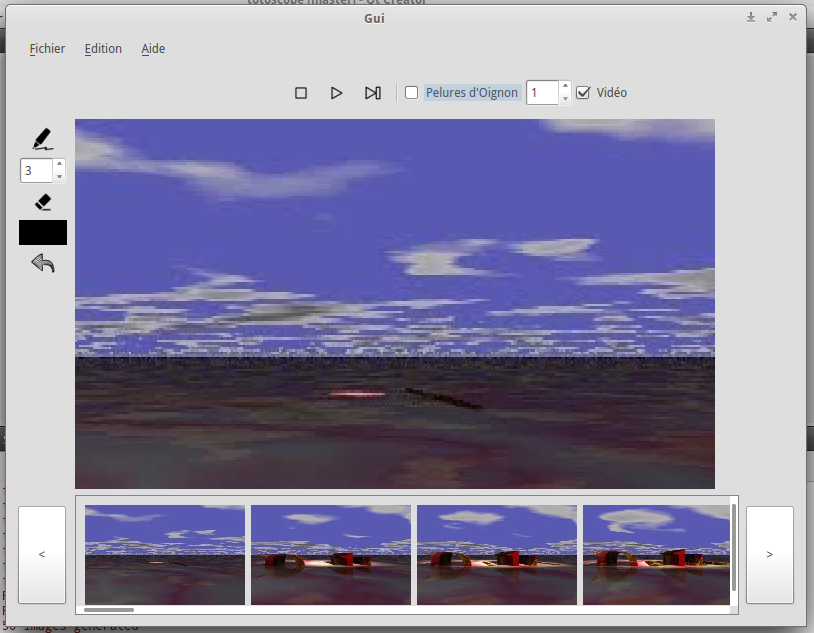
\includegraphics[scale=0.5]{./figures/gui.png}
		\caption{Fenêtre principale de Totoscope}
	\end{figure}

	Notre interface bien que simple et épurée, permet d'effectuer les actions essentielles à l'utilisation du logiciel.
	
	La fenêtre peut être divisée en cinq parties distinctes.
	\subsubsection{La barre de menu principale}
	Elle répertorie toutes les actions possibles de l'application. Elle est fractionnée en trois sous-menus :
	\begin{itemize}
		\item[Fichier] \hfill \\
			Ce menu contient des actions telles que créer un nouveau projet, ouvrir un projet déjà existant, enregistrer ou exporter le travail courant ou encore fermer le projet et le logiciel.
		\item[\'Edition] \hfill \\
			Le menu \'Edition présente les actions fonctionnelles de l'application comme le fait d'annuler la dernière action, ou de la rétablir, l'activation ou non des pelures d'oignon et de la vidéo en arrière plan, et les actions concernant la lecture des dessins déjà effectués.
		\item[Aide] \hfill \\
			Ce menu quant à lui, ne contient que l'action A Propos qui donne accès aux informations concernant l'application.
	\end{itemize}
	
	\subsubsection{La barre de contrôle de la vidéo}
		Elle comprend les actions concernant la vidéo telles que les boutons lecture/pause, stop ou encore image suivante; elle contient aussi les boutons d'activation des pelures d'oignon (ainsi que leur nombre) et de la vidéo en arrière plan.
	
	\subsubsection{La barre latérale de dessin}
		La barre latérale regroupe les différentes actions concernant le dessin comme le crayon ou la gomme, un champ pour leur affecter une taille, la palette de couleur ou encore un bouton pour annuler la dernière action.
	
	\subsubsection{La zone de dessin}
		Elle occupe la part la plus importante de la fenêtre principale puisqu'elle correspond à la fonction première de notre logiciel.
	
	\subsubsection{Les miniatures}
		Les miniatures de la vidéo découpée sont accessibles en partie basse de la fenêtre. Elles permettent une meilleure navigation entre les différentes partie de la vidéo sans encombrer la fenêtre principale.

\subsection{Fenêtre d'exportation}
	La fenêtre d'exportation se divise en deux onglets distincts:
	\subsubsection*{L'exportation au format image}
		Il comprend les options pour l'exportation des dessins au format image. Chaque dessin sera sauvegardé dans un fichier à part dans le dossier mentionné, il sera alors possible de les manipuler grâce à d'autres logiciels.
		
		\begin{figure}[h]
			\centering
			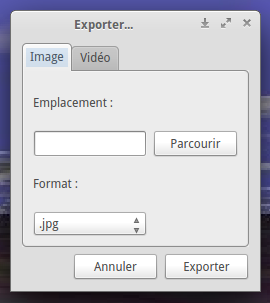
\includegraphics[scale=0.65]{./figures/img.png}
			\caption{Fenêtre d'exportation au format image}
		\end{figure}
	
	\subsubsection*{L'exportation au format vidéo}
		Cet onglet regroupe les options de l'exportation au format vidéo comme l'emplacement du dossier de destination de la vidéo, le codec de la vidéo ou encore son nom.

		\begin{figure}[h]
			\centering
			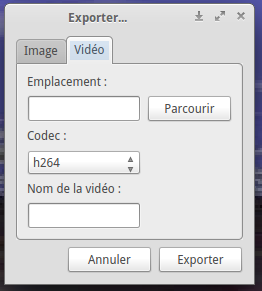
\includegraphics[scale=0.65]{./figures/vid.png}
			\caption{Fenêtre d'exportation au format vidéo}
		\end{figure}